\documentclass[12pt, a4paper]{article}
\setlength{\oddsidemargin}{0.5cm}
\setlength{\evensidemargin}{0.5cm}
\setlength{\topmargin}{-1.6cm}
\setlength{\leftmargin}{0.5cm}
\setlength{\rightmargin}{0.5cm}
\setlength{\textheight}{24.00cm} 
\setlength{\textwidth}{15.00cm}
\parindent 0pt
\parskip 5pt
\pagestyle{plain}

\title{Research Proposal}
\author{}
\date{}

\newcommand{\namelistlabel}[1]{\mbox{#1}\hfil}
\newenvironment{namelist}[1]{%1
\begin{list}{}
    {
        \let\makelabel\namelistlabel
        \settowidth{\labelwidth}{#1}
        \setlength{\leftmargin}{1.1\labelwidth}
    }
  }{%1
\end{list}}

\usepackage{graphicx}
\graphicspath{ {../figs/} }

\begin{document}
\maketitle

\begin{namelist}{xxxxxxxxxxxx}
\item[{\bf Title:}]
	identify functionality in black box systems using neural networks.
\item[{\bf Author:}]
	Johnathan DiMatteo
\item[{\bf Supervisor:}]
	Professor Sebastian Fischmeister
\item[{\bf Degree:}]
	MMath
\end{namelist}

\section*{Background} 
% In this section you should give some background to your
% research area. What is the problem you are tackling, and why is it
% worthwhile solving? Who has already done some work in this area,
% and what have they achieved?
distances - DTW, pearson

clustering algorithms - k means, dbscan, gmm

other - hmm, autoencoders

Useful in many areas.

identify the acceptable input grammar. 
A novel approach to model learning using machine learning.
by sending I2C messages and analyzing the power trace with neural networks.
Uses: black box HIL testing by manufacturers, finding undocumented functionality for security purposes, input grammar for fuzz tests, inputs for polygraph


\section*{Problem Statement} 
%Now state explicitly the hypothesis you aim to
%test. Make references to the items listed in the Reference section
%that back up your arguments for why this is a reasonable
%hypothesis to test, for example the work of Knuth~\cite{knuth}.
%Explain what you expect will be accomplished by undertaking this
%particular project.  Moreover, is it likely to have any other
%applications?

\begin{enumerate}
    \item \textbf{Change Detector}: Given a black box system, determine internal state changes in response to inputs in order to learn the system's behaviour.
    \item \textbf{Input Generator}: Given inputs and knowledge of previous state changes, what should be the next query to the system?
\end{enumerate}

\section*{Method}

\subsection*{System}

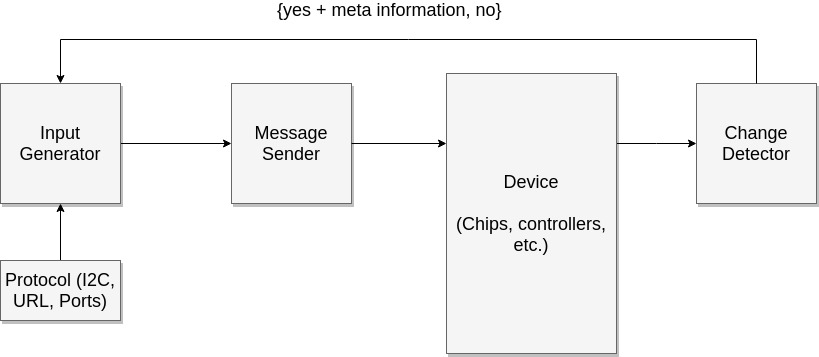
\includegraphics[scale=0.5]{Fuzzer.png}

\subsection*{Change Detector}
distance based: measure of how much the signal moved
dtw: define a threshold. larger difference = more confident.

clustering algorithms: do they require us to input no. of states? online learning? confidence?
options: dbscan, k means
DBSCAN is good, no states required, identifies noise. BUT we have to recalculate with all data points, every time (BUT only do DTW once, ie. 
receive batch of responses, cluster, return yes + msg that triggered it, or no or maybe or more than one + msgs.

Bayesian approach: DETERMINE WHICH CLUSTER OR MAKE A NEW ONE. can eliminate noise manually or just accept it.
for each state, build an expected signal. that way we save out on memory. 
if the expected signal has an extremely high standard deviation ... it might be time to make a new cluster
but we need some way of matching up signals (apparently you can align them using cross correlation, or custom change detection ie. significant change)
compute dtw distance to each expected state signal. (or cluster)
return (current state) or (new state, msg that triggered it)

parameters: eps, min samples, const * standard deviation of expected signals for each state


\subsection*{Input Generator}
L star algorithm: can't because we don't have an oracle that can give us a counterexample, unless we search and depend on our clustering algorithm?
randomization

step 1: determine active msgs.
step 2: try to change the state: send a bunch of messages while modifying one bit at a time depending on protocol (character for URL, bit for NMAP packets).
step 3: receive response from change detector (yes + msg that triggered it, no, maybe, more than one + msgs)

parameters: protocol specification (json?)

\section*{Additional Modules or Functionality}
method to convert states and transitions to mealy machine.
message sender (already implemented for I2C)
focus will be on I2C since system is already in place.

\end{document}


